\section{Analyse et conception d'UC}
On souhaite réaliser un flip flop T dont le symbole est le suivant :
\begin{figure}[h!]
    \begin{center}
        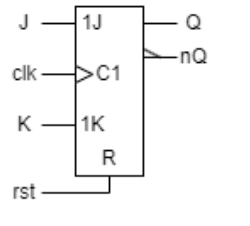
\includegraphics[scale=0.75]{images/Symboles/flipflopJK.png}
    \end{center}
    \caption{Symbole du flip flop JK}
\end{figure}
\newline
La table des fonctions synchrones est la suivante :
\begin{table}[h!]
    \begin{center}
        \begin{tabular}{|c|c|c|}
        \hline
        \textbf{J}  & \textbf{K} & \textbf{Q+} \\
        \hline
        0  & 0 & Q \\
        \hline
        0  & 1 & 0 \\
        \hline
        1  & 0 & 1 \\
        \hline
        1  & 1 & nQ \\
        \hline
        \end{tabular}
    \end{center}    
    \caption{Table de vérité du flip flop JK avec Enable}
\end{table}
\newline
La sortie nQ est simplement l'inverse de Q.
Pour ce faire, il convient de réaliser un schéma bloc du circuit.
\subsection{Schéma Bloc}
\begin{figure}[h!]
    \begin{center}
        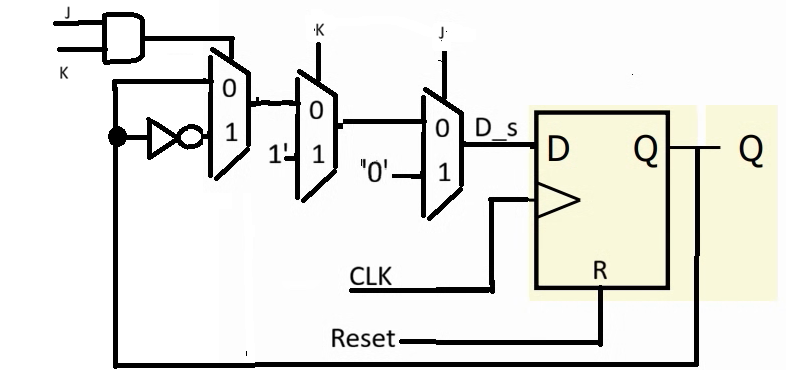
\includegraphics[scale=0.5]{images/SchémaBloc/SchémaBlocJKFF.png}
    \end{center}
    \caption{Schéma bloc du flip flop JK}
\end{figure}
\newpage
D'après la table de vérité, on voit que lorsque K = 0, Q+ vaut not(K),Sinon Q+ vaut J. 
Nous pouvons donc simplifier le schéma bloc de la manière suivante :
\begin{figure}[h!]
    \begin{center}
        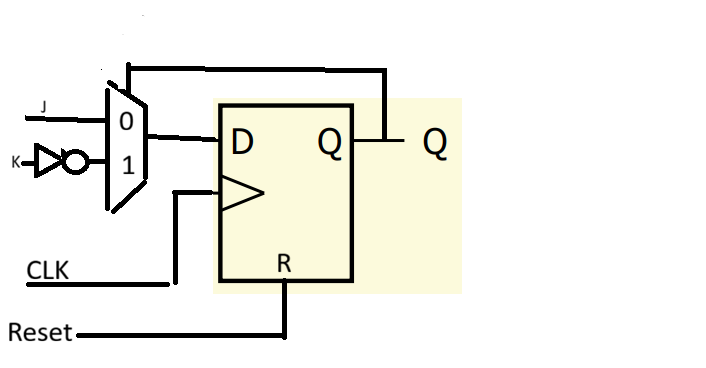
\includegraphics[scale=0.5]{images/SchémaBloc/JKV2_Bloc.png}
    \end{center}
    \caption{Schéma bloc simplifié du flip flop JK}
\end{figure}
\newline
Pour des raisons de manque de temps, nous allons utiliser le premier schéma bloc pour la suite de l'analyse et de la conception du circuit.
\subsection{Description VHDL}
On dispose de l'entité suivante:
\begin{verbatim}
entity flipflop_jk is
   port(clk_i    : in     std_logic;
        reset_i  : in     std_logic;
        J_i      : in     std_logic;
        K_i      : in     std_logic;
        Q_o      : out    std_logic;
        nQ_o     : out    std_logic
   );
end flipflop_jk ;
\end{verbatim}
D'apres le schéma bloc, nous avons les signaux internes suivants :
\begin{verbatim}
    signal reset_s : std_logic;
    signal D_s : std_logic;
    signal Q_s : std_logic;
\end{verbatim}
On a le décodeur d'états présent,donné par le schéma bloc :
\begin{verbatim}
--Adaptation polarite
  reset_s <= reset_i;
  -- Decodeur d'etats present
-- Decodeur d'etats present
  D_s <= not(Q_s) when (J_i = '1' and K_i = '1') else -- Toggle
		 '1' when (J_i = '1') else -- Set
         '0' when (K_i = '1') else -- Reset
          Q_s; -- Maintien
\end{verbatim}
la logique du processus et de la sortie est la même que pour le flip flop D simple :
\begin{verbatim}
  -- Process de bascule
  process(reset_s, clk_i)
  begin
      if reset_s = '1' then
      Q_s <= '0'; -- Etat par défaut
      elsif rising_edge(clk_i) then
      Q_s <= D_s;
      end if;
   end process;
\end{verbatim}
On affecte ensuite les sorties:
\begin{verbatim}
   -- Sorties
   Q_o <= Q_s;
   nQ_o <= not(Q_s);
\end{verbatim}
La description complète du flip flop JK est disponible dans le fichier \textit{src/flipflop\_jk.vhd}.

\subsection{Simulation Automatique}
\begin{verbatim}
# -- Loading package STANDARD
# -- Loading package TEXTIO
# -- Loading package std_logic_1164
# -- Compiling entity flipflop_jk_tb
# -- Compiling architecture test_bench of flipflop_jk_tb
# -- Loading entity flipflop_jk
# ** Warning: ../src_tb/flipflop_jk_tb.vhd(55): (vcom-1236) Shared variables must be of a protected type.
# End time: 11:01:58 on Apr 15,2026, Elapsed time: 0:00:00
# Errors: 0, Warnings: 1
# End time: 11:01:59 on Apr 15,2026, Elapsed time: 0:05:18
# Errors: 0, Warnings: 0
# vsim -voptargs=""+acc"" work.flipflop_jk_tb 
# Start time: 11:01:59 on Apr 15,2026
# ** Note: (vsim-3812) Design is being optimized...
# Loading std.standard
# Loading std.textio(body)
# Loading ieee.std_logic_1164(body)
# Loading work.flipflop_jk_tb(test_bench)#1
# Loading work.flipflop_jk(comport)#1
run -all
# ** Note: >> Debut de la simulation
#    Time: 0 ns  Iteration: 0  Instance: /flipflop_jk_tb
# ** Note: >>Nombre d'erreur détectée = 0
#    Time: 1352 ns  Iteration: 0  Instance: /flipflop_jk_tb
# ** Note: >>Fin de la simulation
#    Time: 1352 ns  Iteration: 0  Instance: /flipflop_jk_tb
\end{verbatim}
\newpage
\subsection{Vue RTL}
\begin{figure}[h!]
    \begin{center}
        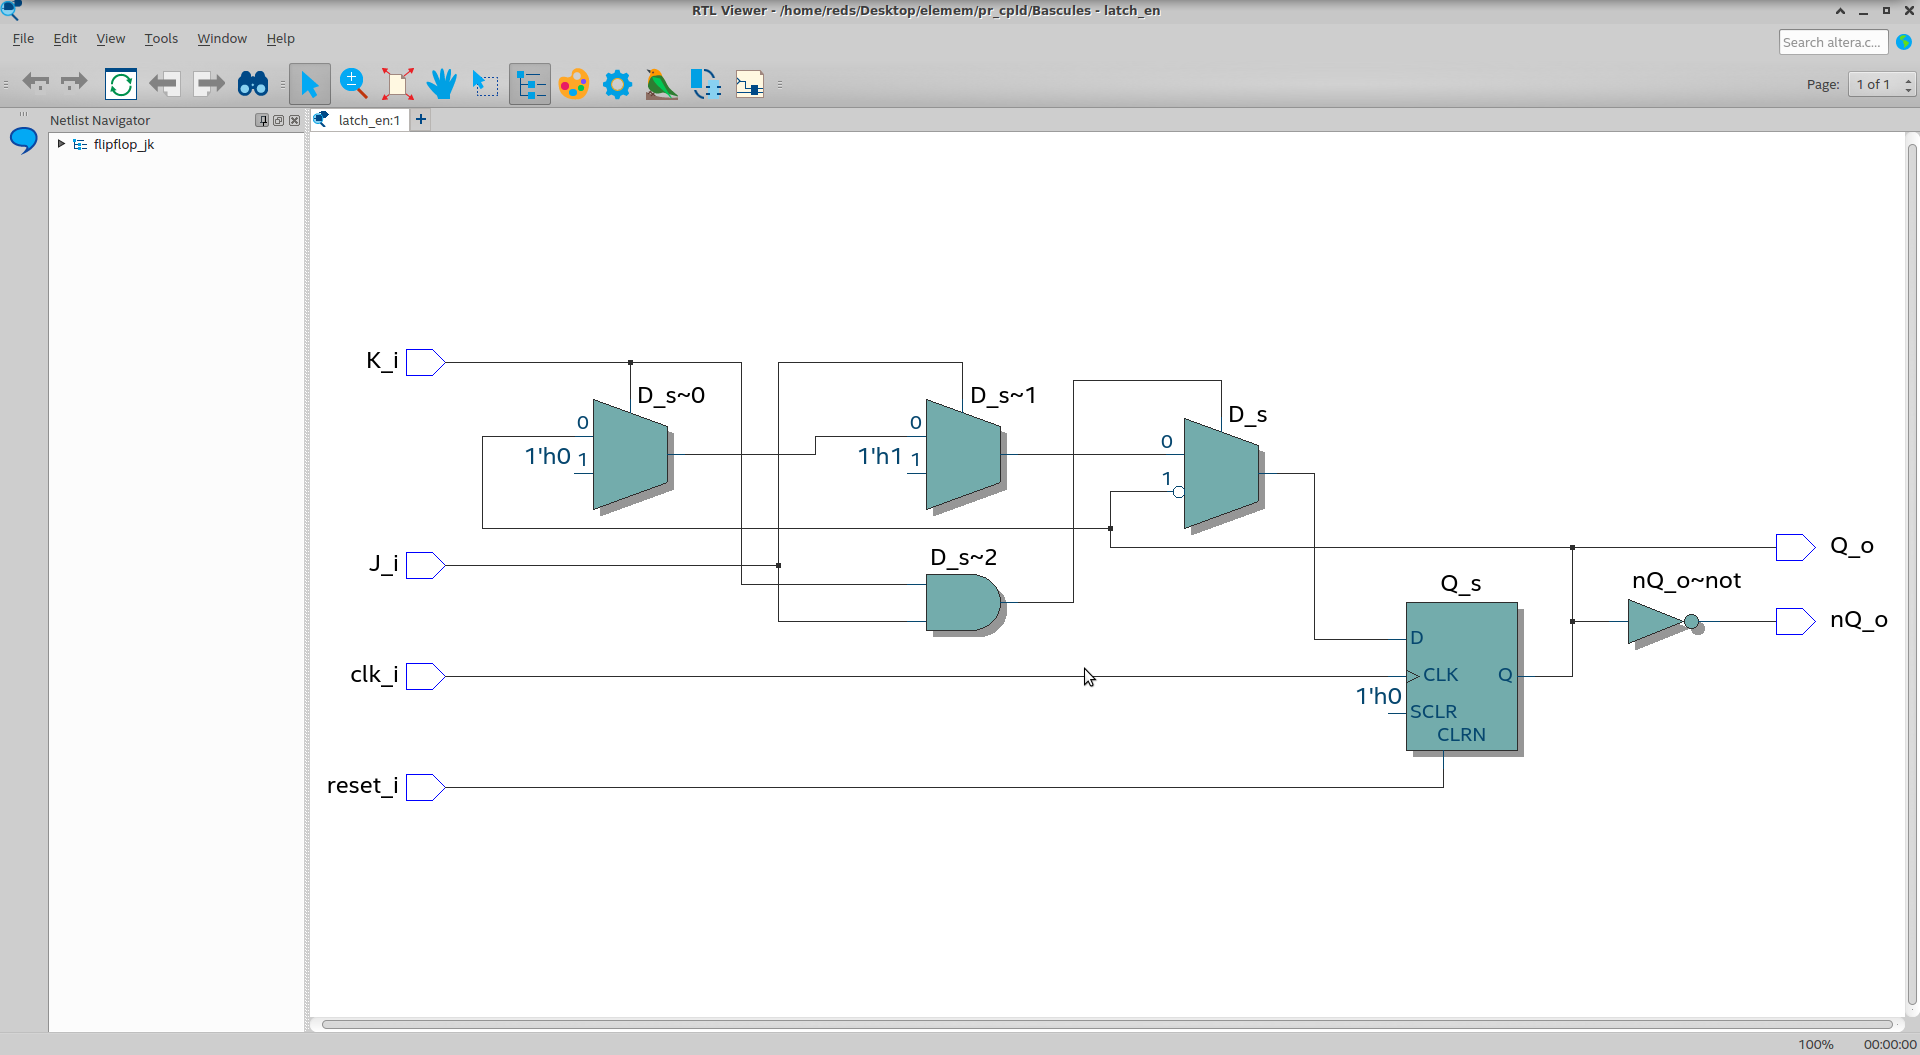
\includegraphics[scale=0.2]{images/VueRTL/jk_VueRTL.png}
    \end{center}
    \caption{Vue RTL du flip flop JK}
\end{figure}
On voit que le décodeur d'états présent est à gauche, la bascule est au centre, et les sorties sont à droite.
La vue RTL correspond bien au premier schéma bloc du flip flop JK.
